\documentclass[12pt,a4paper]{exam}
\usepackage[utf8]{inputenc}
\usepackage[T1]{fontenc}
\usepackage{amsmath}
\usepackage{amsfonts}
%\usepackage{amssymb}
\usepackage{graphicx}
\usepackage{geometry}
\usepackage{enumitem}

\geometry{a4paper, margin=2cm}

\usepackage{cprotect}

\usepackage{xcolor}
\definecolor{maroon}{cmyk}{0, 0.87, 0.68, 0.32}
\definecolor{halfgray}{gray}{0.55}
\definecolor{ipython-frame}{RGB}{207, 207, 207}
\definecolor{ipython-bg}{RGB}{247, 247, 247}
\definecolor{ipython-red}{RGB}{186, 33, 33}
\definecolor{ipython-green}{RGB}{0, 128, 0}
\definecolor{ipython-cyan}{RGB}{64, 128, 128}
\definecolor{ipython-purple}{RGB}{170, 34, 255}
\usepackage{listings}
\lstdefinelanguage{iPython}{
	morekeywords={access,and,del,except,exec,in,is,lambda,not,or,raise},
	morekeywords=[2]{for,print,abs,all,any,basestring,bin,bool,bytearray,callable,chr,classmethod,cmp,compile,complex,delattr,dict,dir,divmod,enumerate,eval,execfile,file,filter,float,format,frozenset,getattr,globals,hasattr,hash,help,hex,id,input,int,isinstance,issubclass,iter,len,list,locals,long,map,max,memoryview,min,next,object,oct,open,ord,pow,property,range,reduce,reload,repr,reversed,round,set,setattr,slice,sorted,staticmethod,str,sum,super,tuple,type,unichr,unicode,vars,xrange,zip,apply,buffer,coerce,intern,elif,else,if,continue,break,while,class,def,return,try,except,import,finally,try,except,from,global,pass, True, False},
	sensitive=true,
	morecomment=[l]\#,%
	morestring=[b]',%
	morestring=[b]",%
	moredelim=**[is][\color{black}]{@@}{@@},
	%%
	%morestring=[s]{'''}{'''},% used for documentation text (mulitiline strings)
	%morestring=[s]{"""}{"""},% added by Philipp Matthias Hahn
	%%
	%morestring=[s]{r'}{'},% `raw' strings
	%morestring=[s]{r"}{"},%
	%morestring=[s]{r'''}{'''},%
	%morestring=[s]{r"""}{"""},%
	%morestring=[s]{u'}{'},% unicode strings
	%morestring=[s]{u"}{"},%
	%morestring=[s]{u'''}{'''},%
	%morestring=[s]{u"""}{"""}%
	%
	% {replace}{replacement}{lenght of replace}
	% *{-}{-}{1} will not replace in comments and so on
	%literate=
	%{\%}{{{\color{ipython-purple}+}}}1,
	%{á}{{\'a}}1 {é}{{\'e}}1 {í}{{\'i}}1 {ó}{{\'o}}1 {ú}{{\'u}}1,
	%{Á}{{\'A}}1 {É}{{\'E}}1 {Í}{{\'I}}1 {Ó}{{\'O}}1 {Ú}{{\'U}}1
	%{à}{{\`a}}1 {è}{{\`e}}1 {ì}{{\`i}}1 {ò}{{\`o}}1 {ù}{{\`u}}1
	%{À}{{\`A}}1 {È}{{\'E}}1 {Ì}{{\`I}}1 {Ò}{{\`O}}1 {Ù}{{\`U}}1
	%{ä}{{\"a}}1 {ë}{{\"e}}1 {ï}{{\"i}}1 {ö}{{\"o}}1 {ü}{{\"u}}1
	%{Ä}{{\"A}}1 {Ë}{{\"E}}1 {Ï}{{\"I}}1 {Ö}{{\"O}}1 {Ü}{{\"U}}1
	%{â}{{\^a}}1 {ê}{{\^e}}1 {î}{{\^i}}1 {ô}{{\^o}}1 {û}{{\^u}}1
	%{Â}{{\^A}}1 {Ê}{{\^E}}1 {Î}{{\^I}}1 {Ô}{{\^O}}1 {Û}{{\^U}}1
	%{œ}{{\oe}}1 {Œ}{{\OE}}1 {æ}{{\ae}}1 {Æ}{{\AE}}1 {ß}{{\ss}}1
	%{ç}{{\c c}}1 {Ç}{{\c C}}1 {ø}{{\o}}1 {å}{{\r a}}1 {Å}{{\r A}}1
	%{€}{{\EUR}}1 {£}{{\pounds}}1
	%
	%{^}{{{\color{ipython_purple}\^{}}}}1
	%{=}{{{\color{ipython_purple}=}}}1
	%%
	%*{-}{{{\color{ipython_purple}-}}}1
	%{*}{{{\color{ipython_purple}$^\ast$}}}1
	%{/}{{{\color{ipython_purple}/}}}1%%
	%{+=}{{{+=}}}1
	%{-=}{{{-=}}}1
	%{*=}{{{$^\ast$=}}}1
	%{/=}{{{/=}}}1,
	%
	identifierstyle=\color{black}\footnotesize\ttfamily,
	commentstyle=\color{ipython-cyan}\footnotesize\itshape\ttfamily,
	stringstyle=\color{ipython-red}\footnotesize\ttfamily,
	keepspaces=true,
	showspaces=false,
	showstringspaces=false,
	rulecolor=\color{ipython-frame},
	frame=single,
	frameround={t}{t}{t}{t},
	%framexleftmargin=6mm,
	%numbers=left,
	%numberstyle=\color{ipython-cyan},
	backgroundcolor=\color{ipython-bg},
	%   extendedchars=true,
	basicstyle=\footnotesize\ttfamily,
	keywordstyle=[2]\color{ipython-green}\bfseries\footnotesize\ttfamily, 
	keywordstyle=\color{ipython-purple}\bfseries\footnotesize\ttfamily
}

\lstdefinelanguage{iOutput} {
	sensitive=true,
	identifierstyle=\color{black}\small\ttfamily,
	stringstyle=\color{ipython-red}\small\ttfamily,
	keepspaces=true,
	showspaces=false,
	showstringspaces=false,
	rulecolor=\color{ipython-frame},
	%frame=single,
	%frameround={t}{t}{t}{t},
	%backgroundcolor=\color{ipython-bg},
	basicstyle=\small\ttfamily,
}

\lstnewenvironment{ipython}[1][]{\lstset{language=iPython,mathescape=true,escapeinside={*@}{@*}}%
}{%
}

\lstnewenvironment{ioutput}[1][]{\lstset{language=iOutput,mathescape=true,escapeinside={*@}{@*}}%
}{%
}

\title{Financial Market Course 23/24\\ Exam}
\author{Prof. Simone Freschi, Prof. Matteo Sani}
\date{$9^{\mathrm{th}}$ January 2024}

%\printanswers
\noprintanswers
\begin{document}
\maketitle
%\addpoints{exam}
\begin{center}
\fbox{\fbox{\parbox{5.5in}{\centering
Answer the questions in the spaces provided. If you run out of room for an answer, continue on the page back.}}}
\end{center}

\begin{center}
\vspace{5mm}
\makebox[0.75\textwidth]{Student's name:\enspace\hrulefill}
\end{center}

\section*{Questions}
\vspace{.5cm}
\begin{questions}
\question Describe the equation for the expected return for a horizon of 1y of a 10y bond (with a coupon \textbf{C}, duration \textbf{D} and convexity \textbf{Conv}) given the expectation of interest rate movements equal to $\delta r$.
\begin{enumerate}[label=(\alph*),font=\itshape]
\item What will happen if the curve is inverted (short rates are higher than long rates) such as in the USA now, if rates remain unchanged from now to the horizon? 
\item what will happen if the curve is upward sloping but there is a parallel shift in 1y time?
\end{enumerate}
\fillwithlines{3cm}
\begin{solution}
%%%% SOLUTION EX 1
\end{solution}

\question Describe the equation for the return attribution model by Brinson, Hood and Beebower (BHB). 
\begin{enumerate}[label=(\alph*),font=\itshape]
\item Explain the difference between Allocation Effect and Security Selection Effect 
\item Imagine that your portfolio is overweight Energy (30\% vs 20\% Benchmark) and the Energy sector is up 15\%. Your energy stocks in the portfolio are up only 5\%. Determine the allocation effect and the selection effect and the overall portfolio result.
\end{enumerate}
\fillwithlines{3cm}
\begin{solution}
%%%% SOLUTION EX 2
\end{solution}

%\question[15] 	Describe the price in real terms and nominal terms of an Inflation Linked Bond.
%\begin{enumerate}
%\item What will happen to the price if nominal rates rise of 1\% and inflation rises of 2\%.
%\item If real rates are 1\% and nominal rates are 5\% (so brekeven inflation is equal to 4\%). What will happen to the Inflation Linked Bond if breakevens go down of 1\% and real rates remain the same? And what will happen to a Nominal Bond with the same maturity?
%
%\end{enumerate}
%\fillwithlines{3cm}
%
%\question[15] Describe the asset swap contract for a coupon bond with coupons equal to \textbf{C} and dirty Price equal to $P(t)$.	
%\begin{enumerate}
%\item What will happen to the price if the spread increase, all the rest being equal? What does it mean in term of credit quality expectation by the market for the bond's issuer?
%\item What is the difference between asset swap spread and \textbf{G-spread} or \textbf{I-spread} calculated in Bloomberg screen?
%\end{enumerate}
%\fillwithlines{3cm}

%\question[20] What is \texttt{numpy} array ?
%\fillwithlines{3cm}
%\begin{solution}
%\texttt{numpy} arrays are array structure more flexible then standard \texttt{python} lists. By using \texttt{numpy} arrays reading and writing items is faster and more efficient.
%\end{solution}

\question What is the output of the below program ?
\begin{ipython}
>>> names = ['Black', 'Scholes', 'Lederman', 'Hull']
>>> print(names[-1][-1])
\end{ipython}
\makeemptybox{3.cm}
%\vspace{\stretch{1}}
\begin{solution}
The output is: 
\begin{ioutput}
l
\end{ioutput}
\end{solution}

\question
How to print in \texttt{python} the sum of the numbers between 5 and 17 included ?
\makeemptybox{3cm}

\begin{solution}
We can print sum of the numbers starting from 5 to 17 using this code:

\begin{ipython}
>>> print (sum(range(5, 18)))
\end{ipython}
\begin{ioutput}
143
\end{ioutput}
\end{solution}

\question A portfolio has a daily return variation distribution as shown in the following figure. The picture also indicates the \textbf{5\% area} under the distribution. 
Based on the graph estimate the \textbf{2 days 95\%-VaR} and the \textbf{1 day 95\%-Expected Shortfall} values. 
Briefly justify the approximate numbers.
\begin{center}
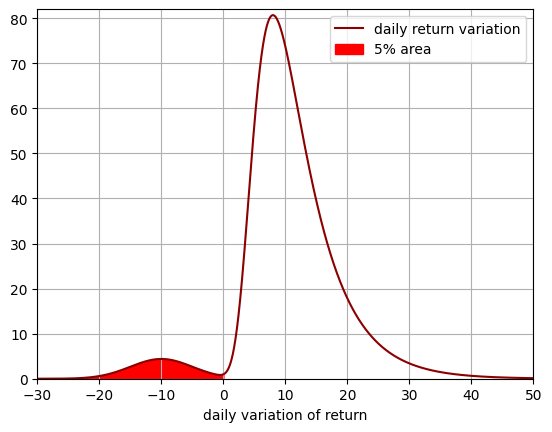
\includegraphics[width=0.8\textwidth]{var2}
\end{center}
\makeemptybox{3cm}

\begin{solution}
2 days 95\%-VaR = $0 \cdot \sqrt{2} \approx 0$, 1 day 95\%-ES $\approx 10$
\end{solution}

\question You have determined the value of an interest rate derivative with a Monte Carlo simulation involving 50 scenarios which results in a contract value of 1.2 M€ $\pm$ 5\%. Unfortunately your boss ask you to determine more precisely the derivative value. If you have to meet him in 1 hour and each simulation lasts about 2.5 sec., what is the highest precision you can achieve ?
\makeemptybox{1.5 cm}

\begin{solution}
Given you have to answer in 1 hour, you can run at most: $\frac{3600}{2.5}=1440$ experiments. Since the result precision scale as the square root of the number of simulations
\begin{equation*}
\textrm{new uncertainty} = 0.05 \cdot \sqrt{\frac{50}{1440}} \approx 0.01
\end{equation*}
\end{solution}

\end{questions}
\end{document}
